%%%%%%%%%%%%%%%%%%%%%%%%%%%%%%%%%%%%%%%%%%%%%%%%%%%%%%%%%% Chap :
\chapter{Références}
\begin{description}
	\item[\pepitSite{}:] site web pepit, portails de jeux éducatifs
	\item[\siteulco{}:] site de l'\ulco
	\item[glossaire:] voir annexe~\ref{annexe_glossaire}
	\item[\href{http://fr.wikipedia.org/}{fr.wikipedia.org}:] encyclopédie dont la réputation n'est plus à faire. Ce site sert pour une bonne partie des \og{}liens informatifs\fg{} dans ce rapport
\end{description}


%%%%%%%%%%%%%%%%%%%%%%%%%%%%%%%%%%%%%%%%%%%%%%%%%%%%%%%%%% Chap :
\chapter{Glossaire}
\label{annexe_glossaire}
\includepdf[page=1]{\dossierpdf Glossaire}


%%%%%%%%%%%%%%%%%%%%%%%%%%%%%%%%%%%%%%%%%%%%%%%%%%%%%%%%%% Chap :
%\chapter{Scripts de réunions}
%\section*{1\iere{} réunion (29/10/2012)}
%\label{reunion1}
%% les includes sont incomplets, il faut préciser la plage de page qu'on importe
%\includepdf{\dossierpdf reunion1_29_10_2012_debut_du_projet}
%\section*{2\ieme{} réunion (26/11/2012)}
%\includepdf{\dossierpdf reunion2_26_11_2012}
%\section*{3\ieme{} réunion (17/12/2012)}
%\includepdf{\dossierpdf reunion3_17_12_2012}


%%%%%%%%%%%%%%%%%%%%%%%%%%%%%%%%%%%%%%%%%%%%%%%%%%%%%%%%%% Chap :
\chapter{Architecture}
\label{annexe_architecture}
\includepdf[page=1-3]{\dossierpdf scenario}


%%%%%%%%%%%%%%%%%%%%%%%%%%%%%%%%%%%%%%%%%%%%%%%%%%%%%%%%%% Chap :
\chapter{Maquettes}
\section*{Maquette - Page d'accueil}
\begin{figure}[H]
\begin{center}
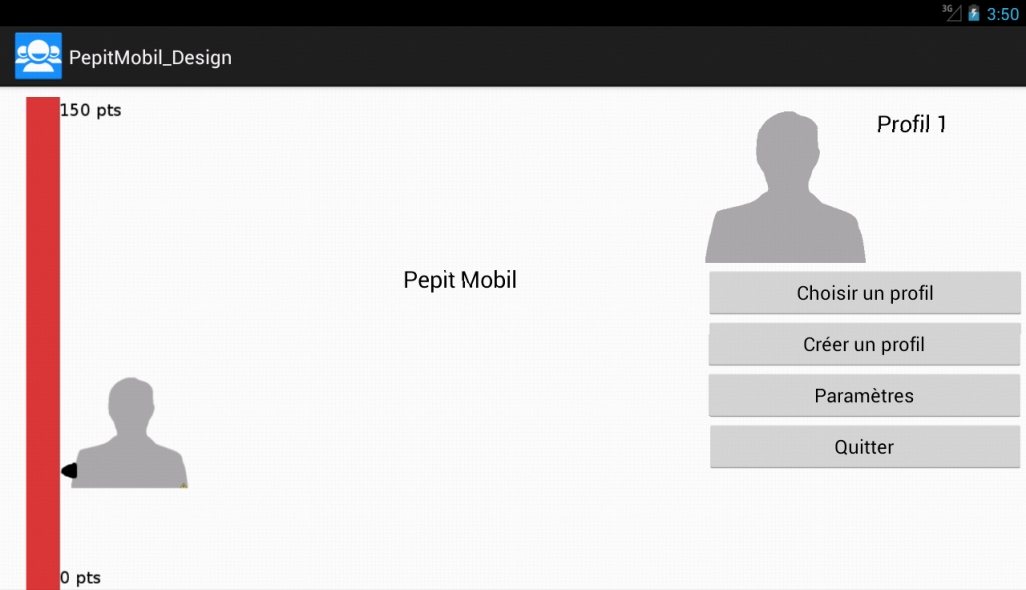
\includegraphics[width=15cm]{images/maquettes_homePage}
\end{center}
\caption{Pepit Mobil - Page d'accueil}
\label{Pepit Mobil - Page d'accueil}
\end{figure}

\section*{Maquette - Exercices}
\begin{figure}[H]
\begin{center}
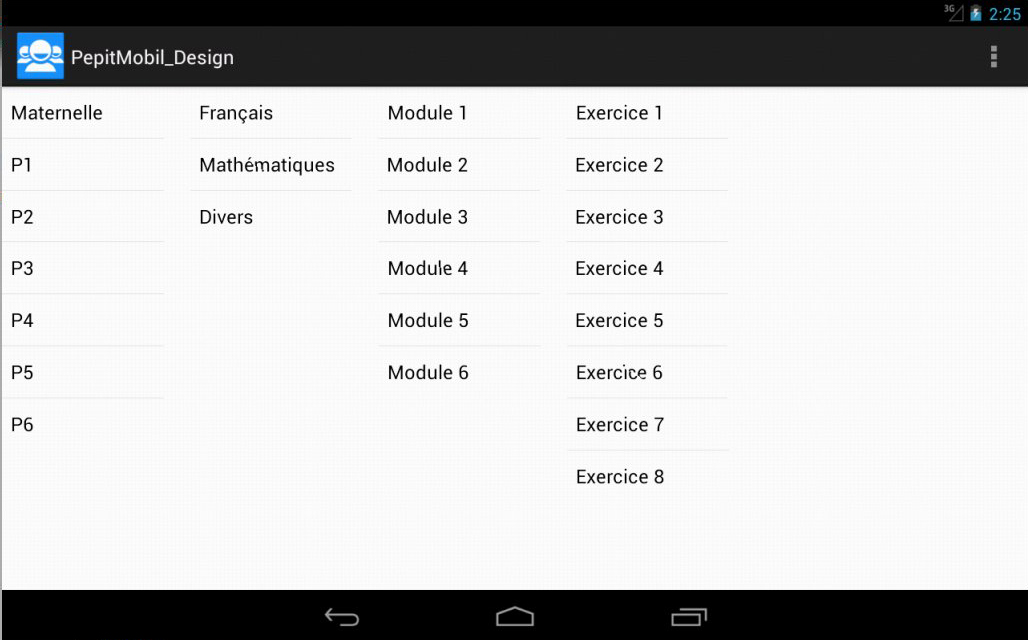
\includegraphics[width=15cm]{images/maquettes_exercices}
\end{center}
\caption{Pepit Mobil - Page exercices}
\label{Pepit Mobil - Page exercices}
\end{figure}

\section*{Maquette - Création de profil}
\begin{figure}[H]
\begin{center}
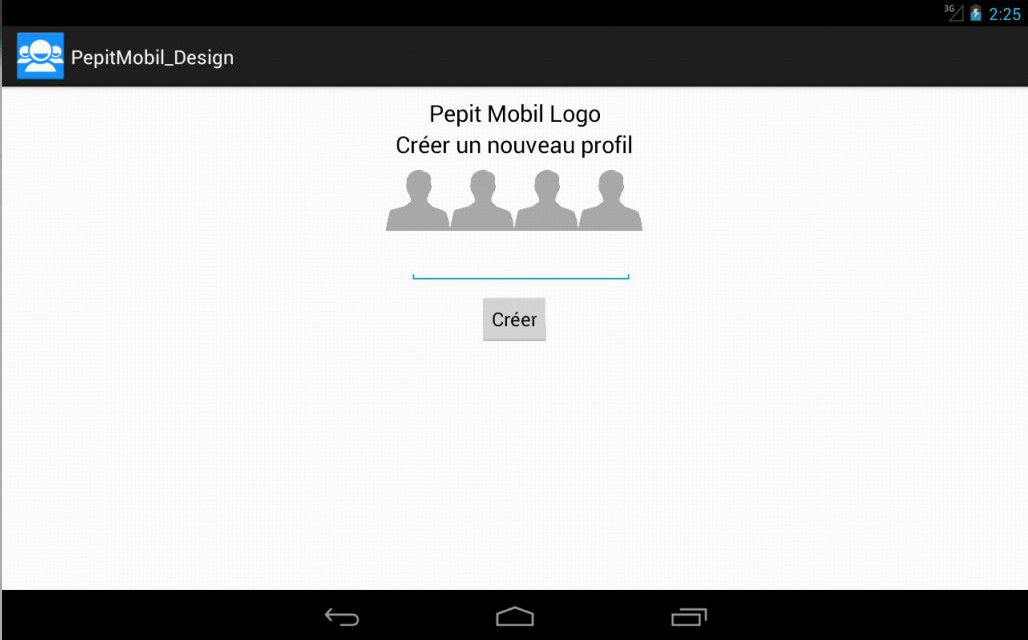
\includegraphics[width=15cm]{images/maquettes_creer_user}
\end{center}
\caption{Pepit Mobil - Page de création de profil}
\label{Pepit Mobil - Page de création de profil}
\end{figure}

\section*{Maquette - Paramètres}
\begin{figure}[H]
\begin{center}
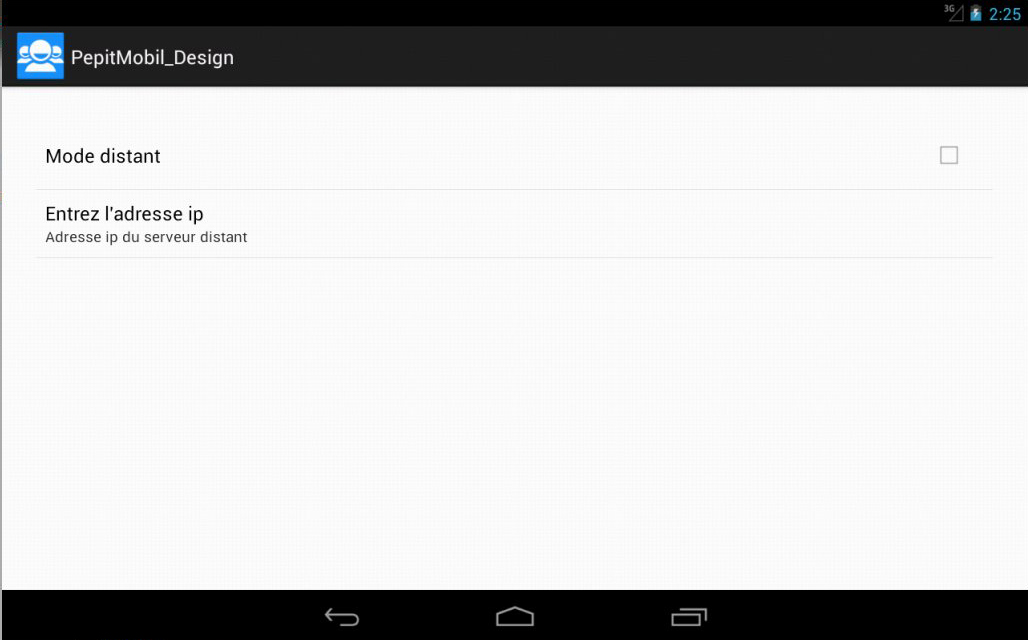
\includegraphics[width=15cm]{images/maquettes_parametres}
\end{center}
\caption{Pepit Mobil - paramètres de l'application}
\label{Pepit Mobil - paramètres de l'application}
\end{figure}